\section{实验}
\label{sec:experiments}
Waymo 实验评价重建精度与轨迹外渲染质量，隐藏表面配对测试与参与者编辑则评价联合补全及固定资产复用。主结果采用中心射线规则 C，足迹规则 F 单独进行受控比较。补充材料附录 A 报告 nuScenes 零样本迁移。




\subsection{实验设置}
\label{sec:experimental_setup}
\paragraph{数据与监督。}
Waymo 的 798 条训练序列拆为 740 条训练和 58 条开发序列，202 条验证序列用于测试。合成训练使用 10,000 个场景、80 张地图、10,000 辆车和 2,500 个人体身份。源地图、车辆基础模型与人体身份先划分，再生成外观／动作变体；真实日志按路段、采集片段及可识别身份隔离。完整划分规模与监督见附录 B。

\paragraph{基线。}
STORM、DGGT 和 StreetForward~\cite{yang2025storm,chen2025dggt,yu2026streetforward} 均随机初始化，在相同真实日志、合成场景和完整资产上重训。各方法使用自身监督目标，Ours 另用单元空域及模板绑定监督。统一状态适配器为预测高斯分配归属并转入规范坐标，用于刚体和骨架放置。所有方法共享上下文 RGB、标定、自车位姿、车辆框／根轨迹及目标人体关节，体型与绑定来自上下文，测试权重固定。训练成本和适配细节见附录 F。

\paragraph{采样与指标。}
每条测试序列取 200 帧，共形成 2,020 个互不重叠的 20 帧、10 Hz 片段。三个前向相机在 $\{0,5,10,15\}$ 提供上下文~\cite{yang2025storm}，其余 12 帧插值与四帧外推共形成 96,960 张目标图像，外推使用给定状态。以 $240\times160$ 图像~\cite{huang2026instantnurec} 计算全图／动态 PSNR 和 SSIM，并在有效 LiDAR 点计算深度 AbsRel/$\delta_1$。深度逐帧尺度对齐后评价，附录 F 同时报未对齐结果；指标按帧、片段、序列依次平均，各序列等权。

\subsection{动态场景重建}
\label{sec:temporal_evaluation}
DriveCompose 在 Waymo 的六项指标上均领先（表~\ref{tab:regions_current}），全图与动态区域 PSNR 分别比 DGGT 高 1.154 和 2.340 dB。结果按 $3{:}1$ 汇总插值与外推，附录 F 分别报告两组结果。图~\ref{fig:dynamic-reconstruction} 显示更清晰的参与者轮廓与道路结构。
\begin{table}[!htbp]
\centering
\footnotesize
\setlength{\tabcolsep}{1.3pt}
\renewcommand{\arraystretch}{1.08}
\setlength{\belowcaptionskip}{5pt}
\caption{\textbf{Waymo 条件重建。}插值与外推以 $3{:}1$ 汇总；完整分组结果见补充材料附录 F。}
\label{tab:regions_current}
\begin{tabular}{@{}lcccccc@{}}
\toprule
& \multicolumn{2}{c}{完整图像} & \multicolumn{2}{c}{\shortstack{动态区域}} & \multicolumn{2}{c}{逐帧尺度对齐深度} \\
\cmidrule(lr){2-3}\cmidrule(lr){4-5}\cmidrule(lr){6-7}
方法 & PSNR $\uparrow$ & SSIM $\uparrow$ & PSNR $\uparrow$ & SSIM $\uparrow$ & AbsRel $\downarrow$ & $\delta_1$ $\uparrow$ \\
\midrule
STORM & 26.380 & 0.826 & 22.100 & 0.624 & 0.178 & 0.741 \\
DGGT & 27.410 & 0.794 & 22.710 & 0.651 & 0.249 & 0.668 \\
StreetForward & 27.010 & 0.818 & 20.919 & 0.592 & 0.197 & 0.759 \\
\midrule
Ours & \textbf{28.564} & \textbf{0.901} & \textbf{25.050} & \textbf{0.862} & \textbf{0.095} & \textbf{0.877} \\
\bottomrule
\end{tabular}
\end{table}
\begin{figure*}[t]
  \centering
  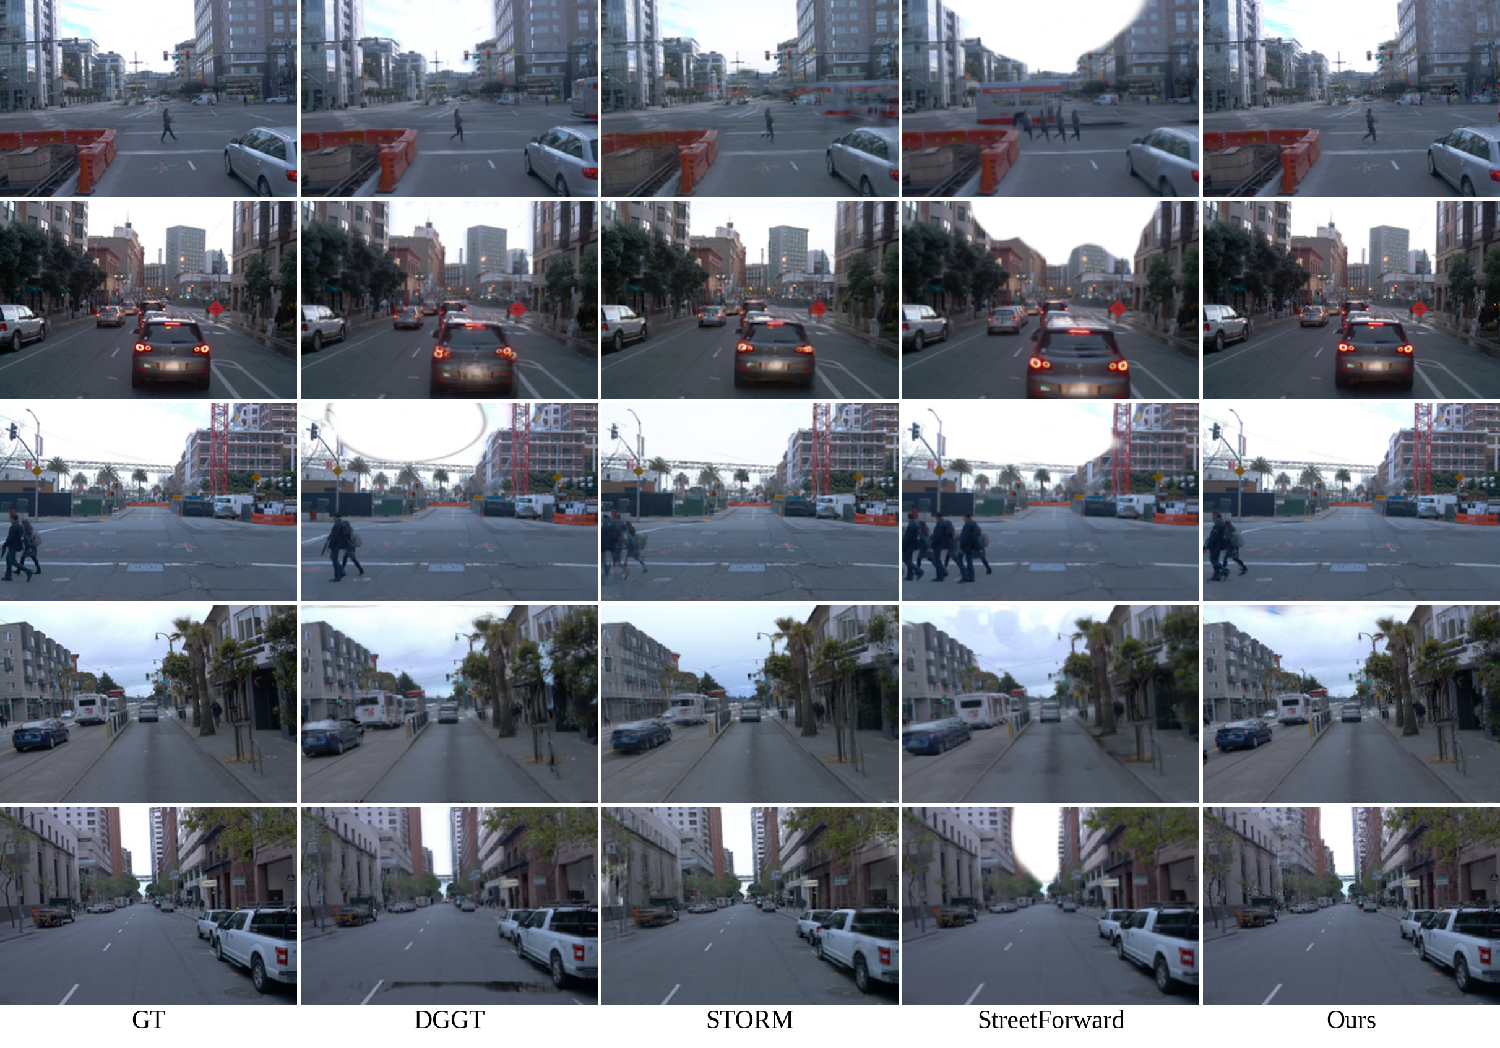
\includegraphics[width=\textwidth]{fig/fig04-dynamic-reconstruction.pdf}
  \caption{\textbf{动态场景条件重建。}每行一个样例，依次为真实目标、DGGT、STORM、StreetForward 与 Ours。}
  \label{fig:dynamic-reconstruction}
\end{figure*}

\subsection{轨迹外渲染}
\label{sec:spatial_evaluation}
相机横向偏移 $\pm1$、$\pm2$、$\pm4$ m，方向、内参和时间戳固定~\cite{chi2026pointforward,zhu2025worldsplat}，比较扩散精修之前的高斯渲染。每个方向包含 121,200 张图像和 6,060 段 20 帧、10 Hz 视频，参考为相同片段、相机与时刻的原轨迹记录。左右方向分别计算 FID 和 FVD 后取均值（表~\ref{tab:spatial_current}；附录 H）。

DriveCompose 在 Waymo 的三种偏移下均取得最低 FID 和 FVD，改善了图像与视频的分布质量（表~\ref{tab:spatial_current}）。图~\ref{fig:waymo-left-shift} 展示偏移渲染及原轨迹参考。

\begin{table}[!htbp]
\centering
\footnotesize
\setlength{\tabcolsep}{2.5pt}
\renewcommand{\arraystretch}{1.08}
\caption{\textbf{离轨视图分布质量。}左右方向分别计算 FID/FVD 后取均值。}
\label{tab:spatial_current}
\resizebox{\columnwidth}{!}{%
\begin{tabular}{@{}l|rr|rr|rr@{}}
\toprule
方法
& \multicolumn{2}{c|}{偏移 $\pm 1$ m}
& \multicolumn{2}{c|}{偏移 $\pm 2$ m}
& \multicolumn{2}{c}{偏移 $\pm 4$ m} \\
\cmidrule(lr){2-3}
\cmidrule(lr){4-5}
\cmidrule(lr){6-7}
& FID $\downarrow$ & FVD $\downarrow$
& FID $\downarrow$ & FVD $\downarrow$
& FID $\downarrow$ & FVD $\downarrow$ \\
\midrule
STORM
& 61.97 & 722.27
& 83.72 & 1029.36
& 132.57 & 1704.16 \\
DGGT
& 73.99 & 984.00
& 93.36 & 1197.03
& 128.01 & 1661.70 \\
StreetForward
& 84.30 & 878.95
& 103.31 & 1095.02
& 123.58 & 1578.63 \\
\midrule
Ours
& \textbf{28.52} & \textbf{544.27}
& \textbf{37.43} & \textbf{673.17}
& \textbf{58.19} & \textbf{817.13} \\
\bottomrule
\end{tabular}%
}
\end{table}
\begin{figure*}[t]
  \centering
  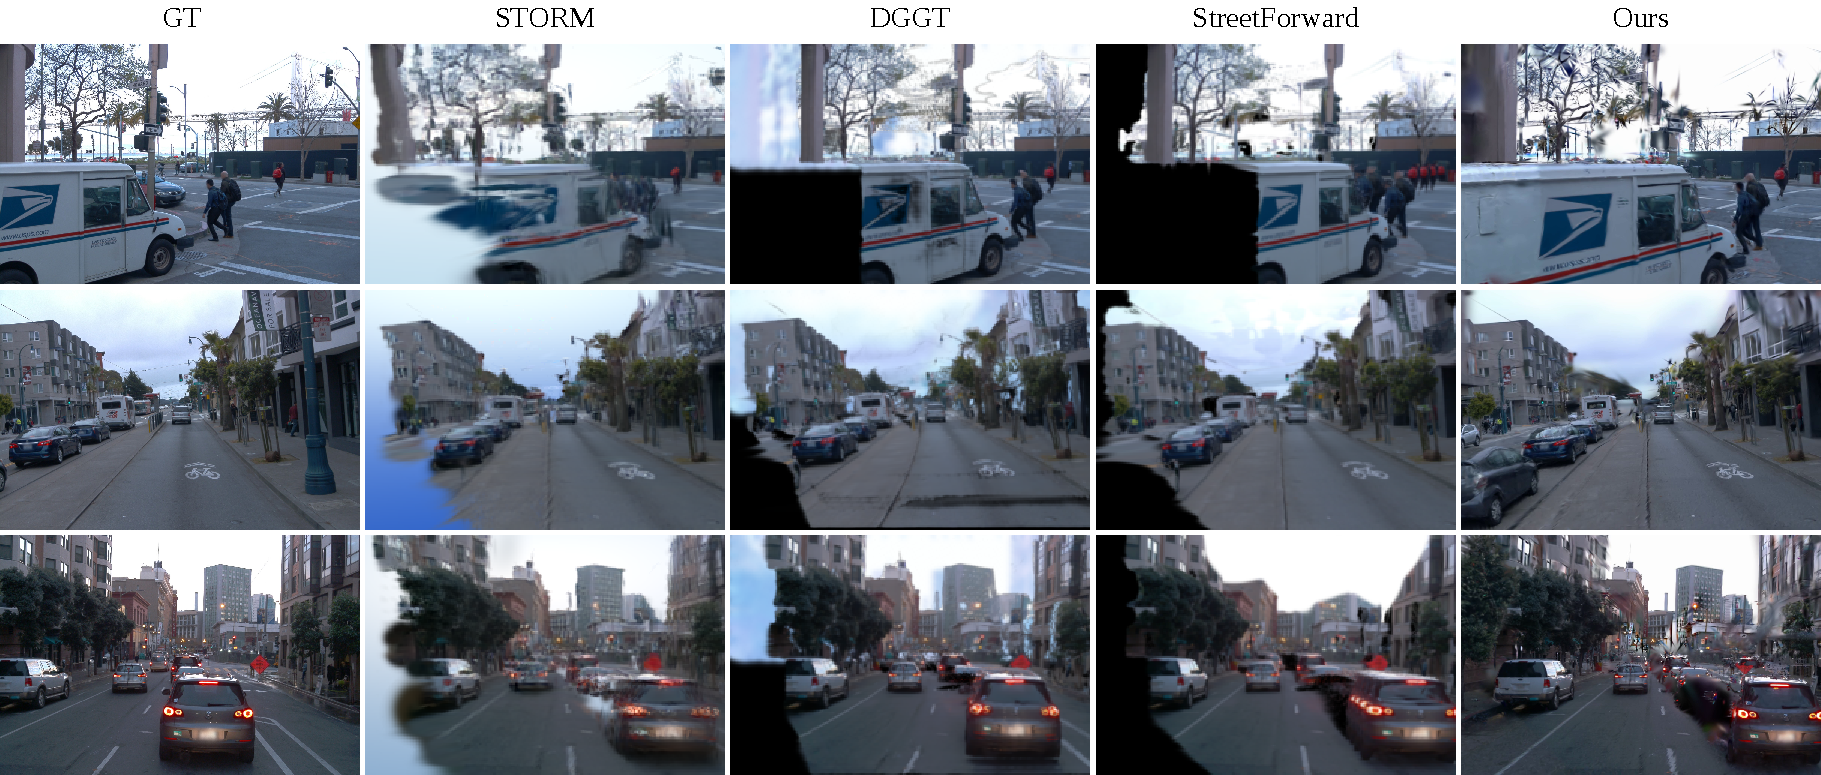
\includegraphics[width=\textwidth]{fig/fig05-off-trajectory-rendering.pdf}
  \caption{\textbf{相机左移 2 m 的离轨渲染。}各列依次为 GT、STORM、DGGT、StreetForward 与 Ours。GT 为原轨迹记录图像。}
  \label{fig:waymo-left-shift}
\end{figure*}


\subsection{状态驱动资产复用}
\label{sec:ablation-reuse}
\paragraph{资产编辑。}
我们在 20 个真实场景上测试固定资产复用，每个场景各含一辆车和一个人体。相机平移 1 m、车辆旋转 $30^\circ$ 及人体换姿均复用固定完成资产。九组训练／生成种子共形成 360 次参与者编辑。五像素结构完整性判据通过 334／360 次（92.78\%）；结构、新增表面纹理、外观身份与局部几何四项联合通过 298／360 次（82.78\%）。五人中至少四人同意的评判规则、失败分解与种子统计见附录 I。

\paragraph{观测保持。}
在固定相机与参与者状态下，相对仅已见场景，Ours 严格保持已见高斯参数，输入视角 PSNR 下降 0.029 dB，深度 MAE 增加 2 mm。人体原已见纹理的规范对应线性 RGB MAE 为 0.014。参数与渲染测量见附录 J。

\paragraph{效率。}
RTX 4090 上（FP16、batch 1、C 规则），构建耗时 $2.66\pm0.11$ s，单相机装配与 $240\times160$ 渲染耗时 $7.8\pm0.4$ ms，峰值显存 14.2 GB。复用已构建资产，1,000 次输出的总成本摊销为每图 10.46 ms。计时条件见附录 K。

% Keep the main qualitative comparisons before the ablation block.
\FloatBarrier
\subsection{消融实验}
\label{sec:ablation-protocol}\label{sec:ablations}\label{sec:ablation-studies}
w/o GCM 关闭非已见、非天空高斯。w/o CCM 使用各组件独立记忆，保留相同参数与全局日志条件，重新训练阶段三、四。

\paragraph{补全组件。}
Waymo 组件消融从每条测试序列取一个 29 时刻窗口，使用三相机、$T=2,4,8$ 嵌套输入与七个共享目标（附录 G）。变体共享恢复模块、codec、状态、数据和优化预算。训练均匀采样 $T$，推理使用 24 步 Euler 积分。三个训练种子与三个生成种子全部平均，所有输出保留计分。交换组件上下文使全图／动态 PSNR 分别提高 0.627／0.934 dB（表~\ref{tab:ablation-components}）；Ours 与 w/o CCM 的训练种子 SD 为 0.061 和 0.074 dB。$T=2,4,8$ 时的 PSNR 增益为 1.104、0.738 和 0.627 dB，输入最稀疏时收益最大（附录 G）。CCM 增加 5.1\% 构建时间（附录 K）。

\begin{table}[!htbp]
  \centering
  \caption{\textbf{Waymo 组件消融。}$T=8$，恢复模块、codec 与目标视图相同。完整 SD 见附录 G。}
  \label{tab:ablation-components}
  \small
  \setlength{\tabcolsep}{3pt}
  \renewcommand{\arraystretch}{1.12}
  \begin{tabular*}{\linewidth}{@{\extracolsep{\fill}}lccccc@{}}
    \toprule
    \multirow{2}{*}{变体} & \multicolumn{3}{c}{全图} & \multicolumn{2}{c}{动态区域} \\
    \cmidrule(lr){2-4}\cmidrule(lr){5-6}
      & PSNR $\uparrow$ & SSIM $\uparrow$ & LPIPS $\downarrow$ & PSNR $\uparrow$ & SSIM $\uparrow$ \\
    \midrule
    w/o GCM & 27.137 & 0.867 & 0.183 & 23.431 & 0.811 \\
    w/o CCM & 28.286 & 0.893 & 0.147 & 24.683 & 0.849 \\
    \midrule
    Ours & \textbf{28.913} & \textbf{0.911} & \textbf{0.129} & \textbf{25.617} & \textbf{0.873} \\
    \bottomrule
  \end{tabular*}
\end{table}

\paragraph{隐藏表面补全。}
\label{sec:hidden-completion}
100 个合成测试场景提供 $\pm2$ m 下的隐藏区域配对评价。场景级潜码生成~\cite{liao2025complete}和跨对象潜码耦合~\cite{wu2026jrm}适配到共享恢复模块、codec、查询布局、输入、监督和采样设置，汇总三个训练种子与三个生成种子。联合补全同时改善外观与表面恢复，相对对象耦合对照的 PSNR、覆盖率和 F-score 分别提高 0.67 dB、2.6 和 3.6 个百分点（表~\ref{tab:completion-mechanisms}）。真实共有支持集上的 RGB 重投影 MAE 相对 w/o CCM 从 0.028 降至 0.019，覆盖率从 86.9\% 升至 92.4\%。机制接口与几何评价见附录 H。

\begin{table}[!htbp]
\centering\small
\setlength{\tabcolsep}{3pt}
\caption{\textbf{隐藏区域补全机制。}100 个合成场景上的任务适配对照，采用 C 规则；覆盖率与 F-score 阈值为 2 cm。}
\label{tab:completion-mechanisms}
\begin{tabular*}{\linewidth}{@{\extracolsep{\fill}}lrrrr@{}}
\toprule
机制 & PSNR$\uparrow$ & LPIPS$\downarrow$ & 覆盖率$\uparrow$ & F-score$\uparrow$\\
\midrule
w/o GCM & 16.82 & 0.401 & 61.5\% & 51.7\%\\
w/o CCM & 21.56 & 0.236 & 89.7\% & 81.3\%\\
场景潜码 & 22.24 & 0.221 & 91.8\% & 84.1\%\\
对象耦合 & 22.51 & 0.212 & 92.4\% & 85.0\%\\
Ours & \textbf{23.18} & \textbf{0.192} & \textbf{95.0\%} & \textbf{88.6\%}\\
\bottomrule
\end{tabular*}
\end{table}

\paragraph{可见率分组分析。}
在 100 个合成场景上，按输入视图并集的表面覆盖率划分充分可见（$\geq80\%$）与严重缺失（$\leq20\%$）组。严重缺失背景／车辆／人体分别获得 1.02／1.28／1.54 dB 增益，充分可见组为 0.04／0.04／0.03 dB。固定 checkpoint 的读取范围干预见附录 H。

\paragraph{编辑后的补全。}
在 20 个身份隔离合成场景上执行第~\ref{sec:ablation-reuse} 节的相同编辑，每个场景各含一辆车和一个人体。联合补全在新增可见表面的 PSNR、LPIPS 和覆盖率上均取得最优结果（表~\ref{tab:asset-reuse}）。

\begin{table}[!htbp]
\centering\small
\setlength{\tabcolsep}{1.5pt}
\caption{\textbf{编辑后新增可见资产表面。}合成配对测试中的补全消融，车辆／人体覆盖阈值为 2／1 cm。}
\label{tab:asset-reuse}
\begin{tabular*}{\linewidth}{@{\extracolsep{\fill}}lrrrrrr@{}}
\toprule
变体 & \multicolumn{3}{c}{车辆（2 cm）} & \multicolumn{3}{c}{人体（1 cm）}\\
\cmidrule(lr){2-4}\cmidrule(lr){5-7}
& PSNR$\uparrow$ & LPIPS$\downarrow$ & Cov.$\uparrow$ & PSNR$\uparrow$ & LPIPS$\downarrow$ & Cov.$\uparrow$\\
\midrule
w/o GCM & 17.80 & 0.362 & 63.4\% & 17.12 & 0.391 & 60.8\%\\
w/o CCM & 22.46 & 0.218 & 91.8\% & 21.38 & 0.247 & 88.6\%\\
Ours & \textbf{24.18} & \textbf{0.176} & \textbf{96.1\%} & \textbf{23.06} & \textbf{0.201} & \textbf{94.3\%}\\
\bottomrule
\end{tabular*}
\end{table}

\paragraph{自由空间约束。}
\label{sec:observation-preservation}
在 2,020,000 条固定射线上，新增遮挡及严格自由射线违规率为 0.18\% 和 0.07\%；移除自由射线损失后增至 1.34\% 和 0.91\%（附录 J）。固定权重、布局、深度与逐查询噪声，F 将含表面单元误标从 1,374 个降至 19 个。隐藏区域覆盖率从 95.0\% 增至 96.2\%，PSNR 从 23.18 增至 23.36 dB，构建时间从 2.66 增至 2.86 s。单元误标、表面覆盖与射线违例分别报告于附录 D。
\FloatBarrier
